\section{The Standard Model}

%The Standard Model of particle physics is a theory that describes fundamental particles and their interactions.
%In the standard model physical phenomena are made up of the fundamental particles or compositions of fundamental particles.
%The fundamental particles are classified into quarks, leptons, gauge bosons and the Higg's boson.
%Fundamental particles are classified into fermions and bosons based on their intrinsic property of spin.
%Fermions are further subdivided into leptons and quarks.
%Both leptons are quarks have three generations.
%Bosons are subdivided into gauge bosons and the Higg's boson.
%Gauge bosons mediate interactions between particles.

The Standard Model %of particle physics is a theory that% 
describes fundamental particles and their interactions mediated via force carrying particles. It describes electromagnetism, the weak force and the strong force. 

%Gravity is not incorporated into the standard model though in many cases the gravitational interaction between particles is very small with respect to the other three fundamental forces. For example at the atomic scale the  in these situations the Standard Model has consistently made accurate predictions.

The Standard Model is built upon the principles of Quantum Field Theory and renormalizable gauge theories developed in the twentieth century \cite{Griffiths:Introduction-to-elementary-particles}. It is most commonly represented in the form of the Lagrangian formalism and is divided into the following sectors. The Electroweak sector - describing both electromagnetic forces and weak interactions, Quantum Chromodynamics (QCD) sector - describing the strong interaction and the Higg's sector - describing interactions with the Higg's field.

The Standard Model has proven to be an extremely successful theory having exceptional predictive powers - the theoretical prediction of the electron anomalous magnetic moment being in agreement with experimental data to 10 significant figures \cite{PhysRevLett.97.030801}. 


%Interactions between particles are interpreted as being a result of the exchange of force mediating particles - the gauge bosons mentioned in the previous section. The Standard Model describes interactions between particles as being either via electromagnetic, strong or weak forces. These forces are described by the following theories: the Electroweak theory and Quantum Chromodynamics. In general electromagnetic and weak interactions are described together by the Electroweak theory which is a unification of their respective theories. These theories are built on the framework of quantum field theory. Gravity is not included in the Standard model due to its non-renormalisability as a quantum field theory.
%
%Quantum Electrodynamics describes the electromagnetic force as being the result of the exchange of photons between charged particles, this is an extremely successful theory which exhibits some of the most accurate predictions of any theory. The strong force is most well known for its role in holding nucleons together in the nucleus of the atom, this described by the theory of Quantum Chromodynamics; the strong force is mediated via gluons. The weak interaction is most well known for its role in the process of beta decay; it is mediated by the W and Z gauge bosons. The electromagnetic and weak interactions care together be described the Electroweak theory, this theory incorporates parts of QED and weak interaction physics together with the concept of Electro-Weak Symmetry Breaking. This theory describes electromagnetic and weak interactions as originating from the same force, the process of the electro-weak symmetry breaking causes this force to manifest itself as these two components. Finally the Higg's particle interacts with certain particles, giving rise to the property of massive particles via the Higg's mechanism.

\subsection{Fundamental Particles}

The fundamental particles are categorised by several intrinsic properties which can be seen in table \ref{fig: particle table}. By their intrinsic spin they are classified as particles with half-integer spin (fermions) and integer spin (bosons), these are outlined in the following sections.

\subsection*{Fermions}
Fermions are further sub-divided into two groups - quarks and leptons - depending on the types of interactions they experience. Quarks have the property of colour which makes them sensitive to the strong interaction whilst leptons do not. 

Both quarks and leptons are further sub-divided into three generations; the higher generations correspond to particles with higher mass states, these particles rapidly decay to the lower stable generations by the weak force. 

Each fermion generation consists of a particle doublet, for example the first generation of quarks is composed of up and down type quarks. Particles in fermions doublets couple strongly to one another such that interactions between the two particle types are relatively strong in comparison to coupling between particles in different generations. This can be seen in the CKM matrix (a matrix which describing coupling between different quark types measured through experiment) where the coupling between the �up� and �down� quarks is  approximately four times greater than between �up� and �strange� type quarks. 

The lepton generations are made up of a charged lepton and neutrino doublet. There is no coupling between lepton generations (in contrast to quarks) in the standard model; higher generation lepton states such as the tau lepton may decay via tree processes such as a decay to its corresponding neutrino along with a $\mathrm{W}^\pm$ boson (see subsection below).

The three generations together with the corresponding doublets gives a total of 6 quark flavours and 6 lepton flavours.

\subsection*{Bosons}
The Standard Model describes two types of bosons, gauge bosons and the Higg's boson. 

A gauge boson is a force carrying particle - also referred to as a force mediator - associated to a particular type of interaction e.g. gluons are associated with the strong interaction and photons are associated to the electromagnetic interaction. The term ``gauge'' comes from the property of the equations of motion related to a given interaction; these are invariant under ``gauge'' transformations which are discussed in section \ref{section: gauge theories}.

The Higg�s boson plays a unique role in the Standard Model. Its existence supports the validity of the Higg�s mechanism; a mechanism which explains why some particles are massive while others are not, in addition to why interaction strengths vary for different interaction types. On the 4th July 2012 the discovery of particle with a mass between 125 and 127 GeV was announced; on the 14th March 2013 the properties of the newly discovered particle were found to be consistent with the Higg�s Boson predicted by the standard model.

\begin{figure}[h]
	\centering
	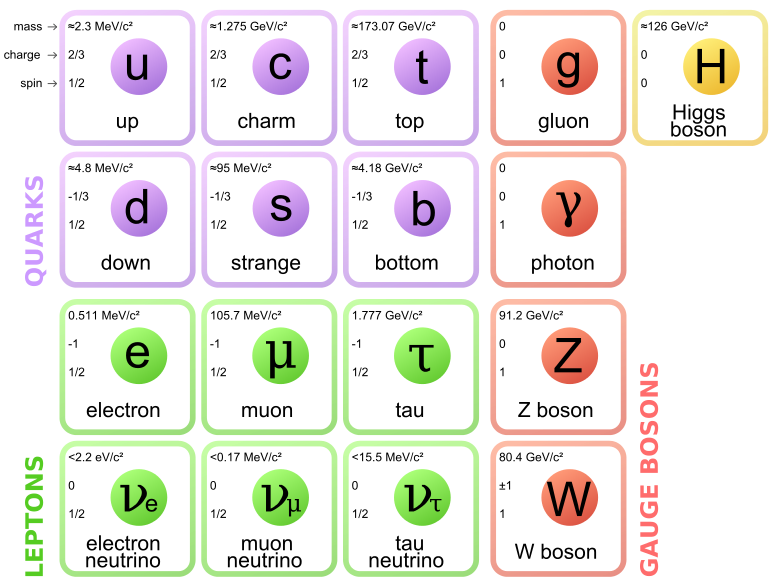
\includegraphics[width=0.75\textwidth]{./Chapters/theory/standard_model/images/particle_table.png}
	\caption{Table of particles in the Standard Model \cite{particle_table}}
	\label{fig: particle table}
\end{figure}
%%\subsection*{Interactions}

%\subsection{Electromagnetism}

The standard model describes the electromagnetic force as being the result of the exchange of photons between charged particles. This interaction is described by the theory of Quantum Electrodynamics (QED), an extremely successful theory which exhibits some of the most accurate predictions of any theory. 
%\subsection{Strong Interaction}
%\subsection{Weak Interaction}
%\subsection{Electroweak Interaction}

\subsubsection{The Higg's Mechanism}
%\subsection{The Higg's Mechanism}
\subsection{Quantum Field Theory (QFT)}

Quantum field theory is built on concepts from Quantum Mechanics, Special Relativity and Classical Field Theory. Fundamental particles are described as excitations or quanta of the fields. For example, electrons are quanta of the electron field and similarly photons are quanta of the electromagnetic field i.e. interactions between electrons can be described as being a result of the interaction between the electron field and electromagnetic field. Mathematically these interactions can be described using the Lagrangian Formalism. 

\subsubsection{Lagrangian Formalism}
With Lagrangian mechanics the equations of motion for a given field is derived by minimising the action $\mathcal{S}$ given by,

\begin{equation}
	\mathcal{S} = \int\mathcal{L}(\phi, \partial_\mu \phi) \mathrm{d}^4x
\end{equation}

where $\mathcal{L}$ is the Lagrangian density, $\phi$ is the field and $\partial_\mu$ is the differential operator acting on the space and time coordinates of the field as seen in special relativity. By applying the condition of the Principle of Least Action, the equations of motion are given by the Euler-Lagrange equation,

\begin{equation}
	\partial_\mu(\frac{\partial\mathcal{L}}{\partial(\partial_\mu\phi_i)}) = \frac{\partial\mathcal{L}}{\partial\phi_i}
\end{equation}

\subsection{Gauge Theories}
\label{section: gauge theories}

A gauge theory is defined by a Lagrangian which is invariant under continuous local transformations of the fields or coordinates. 

\begin{equation}
	\delta \mathcal{L} = 0
\end{equation}

Each possible gauge transformations can be represented by a matrix; together these matrices form a group under matrix multiplication - the symmetry group of the gauge theory.

For each generator of the group there is an associated gauge field, for example, in QED there is one generator to the U(1) group which is associated to the electromagnetic four-vector potential field. Similarly, in QCD there are 8 generators associated to the SU(3) group corresponding to 8 gluon fields. The quanta of the gauge fields are called gauge bosons, for the previous examples these are the photon and gluons respectively.

The symmetry group for the Standard Model is U1 x SU(2) x SU(3), it is a non-Abelian group with 12 gauge fields; the corresponding gauge bosons are the photon, W+, W-, Z0 and eight types of gluon.

%\subsection{Coupling Constants}

The coupling constants of a theory are dimensionless values that describe the strength of an interaction. For example the fine structure constant of QED ($\alpha$) describes the strength of the electromagnetic interaction, defined as,

\begin{equation}
	\alpha = \frac{e^2}{4\pi}
	\label{equation: fine structure constant}
\end{equation}

where $e$ is the charge of the positron\footnote{Expressed in Heaviside-Lorentz and natural units. Unless explicitly stated otherwise all following equations will be expressed in this way} and $\alpha$ has the value $1/137$. Theories with coupling constants that have a value much less than one are said to be weakly coupled. The evolution of systems described by these theories are compatible with perturbative calculations in which the expansion is based on powers of the coupling constant. Conversely theories with coupling constants that have a value of the order of one or greater are said to be strongly coupled and are not compatible with the perturbation method.

The Standard model consists of theories with running coupling constants, which vary depending on the energy scale of a process. The behaviour of these are described by the $\beta$ functions,

\begin{equation}
	\beta(g) = \frac{\partial{g}}{\partial{log(\mu)}}
\end{equation}

where g is the coupling constant of the theory ($g = e$ for QED) and $\mu$ is the interaction energy scale. A $\beta$ function with positive values describes a coupling that increases with the energy of the process and vice-versa. 
\subsection{Coupling Constants}

The coupling constants of a theory are dimensionless values that describe the strength of an interaction. For example the fine structure constant of QED ($\alpha$) describes the strength of the electromagnetic interaction, defined as,

\begin{equation}
	\alpha = \frac{e^2}{4\pi}
	\label{equation: fine structure constant}
\end{equation}

where $e$ is the charge of the positron\footnote{Expressed in Heaviside-Lorentz and natural units. Unless explicitly stated otherwise all following equations will be expressed in this way} and $\alpha$ has the value $1/137$. Theories with coupling constants that have a value much less than one are said to be weakly coupled. The evolution of systems described by these theories are compatible with perturbative calculations in which the expansion is based on powers of the coupling constant. Conversely theories with coupling constants that have a value of the order of one or greater are said to be strongly coupled and are not compatible with the perturbation method.

The Standard model consists of theories with running coupling constants, which vary depending on the energy scale of a process. The behaviour of these are described by the $\beta$ functions,

\begin{equation}
	\beta(g) = \frac{\partial{g}}{\partial{log(\mu)}}
\end{equation}

where g is the coupling constant of the theory ($g = e$ for QED) and $\mu$ is the interaction energy scale. A $\beta$ function with positive values describes a coupling that increases with the energy of the process and vice-versa. 
\subsection{Quantum Electrodynamics (QED)}

QED is an example of a Quantum Field Theory, it describes the electromagnetic interactions between charged fermions via the exchange of photons - gauge bosons of the theory. It is both a Quantum Field Theory as well as a Gauge Theory with a symmetry group of U(1) - an Abelian group of composed of 1 x 1 unitary matrices. The Electroweak theory of the standard model is a unification of QED and Quantum Flavour Dynamics - a gauge theory which describes the weak interaction. The Lagrangian for the QED is given by,

\begin{equation}
	\mathcal{L} = \bar{\psi} (i\gamma^\mu D_\mu - m)\psi - \frac{1}{4}F_{\mu\nu}F^{\mu\nu}
\end{equation}

where $\psi$ is a bispinor field of spin $1/2$ corresponding to the electron field; $\gamma^\mu$ are the Dirac Matrices; $\bar{\psi}$ is the Dirac adjoint spinor $\psi^\dagger \gamma^0$; $D_\mu$ is the gauge covariant derivative given by,

\begin{equation}
	D_\mu = \partial_\mu + ieA_\mu + ieB_\mu
\end{equation}

$e$ is the coupling constant between the electron and electromagnetic fields - charge of an electron; $A_\mu$ is the covariant four-potential of the electromagnetic field generated by the electron; $B_\mu$ is the external field due to an external source and $F_{\mu\nu}$ is the electromagnetic field tensor given by,

\begin{equation}
	F_{\mu\nu} = \partial_\mu A_\nu - \partial_\nu A_\mu
\end{equation}

\subsection{Quantum Chromodynamics (QCD)}

% OVERVIEW
%
%   * a theory of the strong interaction (color force)
%   * It is the study of the SU(3) Yang�Mills theory of color-charged fermions (the quarks)  
%   * Described by the SU(3) group
%   * QCD is a gauge theory of the SU(3) gauge group obtained by taking the color charge to define a local symmetry. 


QCD is a physical theory that describes the interactions between particles with the property of colour via strong interactions. It is a gauge theory with a symmetry group of SU(3) (the group of unitary matrices with a determinant of one) and describes the interactions between quark and gluon fields. 

The strong force is responsible for the binding force which holds nucleons together to form the nucleus of an atom. This is due to the deeper fundamental interaction between the components of nucleons - quarks and gluons - collectively called partons. The gluons are the gauge bosons of the theory i.e. mediators of the strong force. It is a short range force having a significant effect only on scale of $\sim1$ fm (about the size of the charge radius of a proton) due to the nature of its coupling. The Lagrangian of QCD is,

\begin{equation}
	\mathcal{L} = \bar\psi_i i((\gamma^\mu D_\mu)_{ij} - m \delta_{ij})\psi_j - \frac{1}{4}G^a_{\mu\nu}G^{\mu\nu}_a
	\label{equation: qcd lagrangian}
\end{equation}

where $\bar\psi_i$ is the quark field and $G^a_{\mu\nu}$ is the gluon field strength tensor given by,

\begin{equation}
	G^a_{\mu\nu} = \partial_\mu A^a_\nu - \partial_\nu A^a_\mu + gf^{abc} A_\mu^b A_\nu^c
\end{equation}

where $A^a_\nu$ are the gluon fields and $f^{abc}$ are the fine structure constants of the SU(3) group.

%BOUND STATES
Quarks have been observed in two-quark bound states (mesons) and three-quark bound states (baryons); the six flavours of quarks give rise to many possible quark combinations, these combinations are commonly grouped into octets by the eightfold way, figure \ref{fig: eightfold way}.


%\subsection*{Parton Bound States}
%The three colours form a quark triplet, 

%\begin{equation}
%	c = \[
%	\left(
%	\begin{array}{c}
%		\psi_1 \\
%		\psi_2 \\
%		\psi_3   
%	\end{array}
%	\right)
%	\]
%\end{equation}

\begin{figure}[h]
	\begin{subfigure}[h]{0.49\textwidth}
		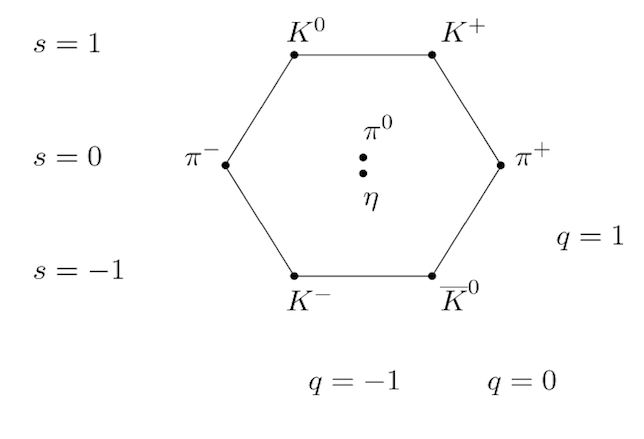
\includegraphics[width=\textwidth]{./Chapters/theory/standard_model/images/meson_octet.png}
		\caption{The meson octet (two quark bound states)}
		\label{fig: meson octet}
	\end{subfigure}
	\begin{subfigure}[h]{0.49\textwidth}
		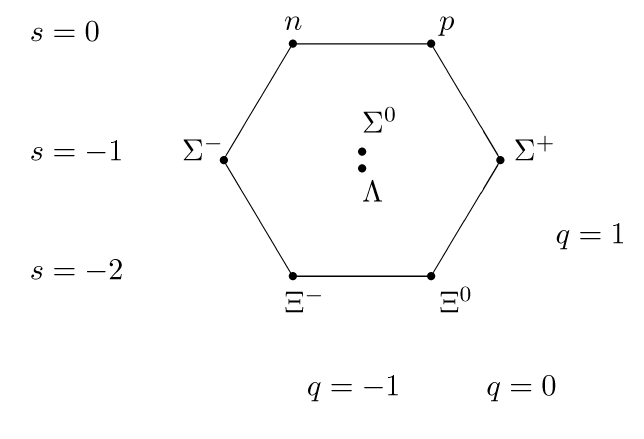
\includegraphics[width=\textwidth]{./Chapters/theory/standard_model/images/baryon_octet.png}
		\caption{Baryon octet (three quark bound states)}
		\label{fig: baryon decuplet}
	\end{subfigure}
	\caption{Eightfold method of organising quark bound states. Bound states on the same horizontal share the same strangeness and those on the same diagonals running top left to bottom right share the same charge}
	\label{fig: eightfold way}
\end{figure}

% COLOUR
The property of colour in QCD is analogous in many ways to the role of electric charge in QED. However instead of there being one type of charge in QCD there are three types, labelled red, green, blue and their corresponding anti-colours anti-red, anti-green and anti-blue. The names of the charge types are motivated by the behaviour of coloured light such that a bound state of a red, blue and green quarks gives a net colour charge of white or colourless; a combination of colour and anti-colour is also colourless.

% PARTONS
Each quark possesses one of the three types of colour charge; it can be either red, green or blue (similarly so for anti-quarks and the anti-colour charges). Gluons on the other hand possess a combination of colour and anti-colour charge (though these charges are not necessarily of the same colour). Since gluons are charged, QCD features some additional richness not seen in its QED counterpart. Gluons can couple with one other unlike photons which cannot, see figure \ref{fig: qcd field couplings}.

\begin{figure}[h]
	\centering
	\begin{subfigure}[h]{0.32\textwidth}
		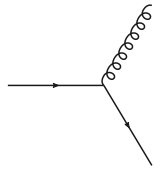
\includegraphics[width=0.8\textwidth]{./Chapters/theory/standard_model/images/quark_gluon.png}
		\caption{Quark-gluon vertex}
		\label{fig: quark-gluon vertex}
	\end{subfigure}
	\begin{subfigure}[h]{0.32\textwidth}
		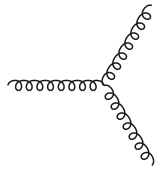
\includegraphics[width=0.8\textwidth]{./Chapters/theory/standard_model/images/gluon3.png}
		\caption{Three-gluon vertex}
		\label{fig: three-gluon vertex}
	\end{subfigure}
	\begin{subfigure}[h]{0.32\textwidth}
		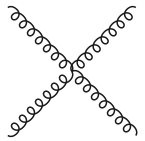
\includegraphics[width=0.8\textwidth]{./Chapters/theory/standard_model/images/gluon4.png}
		\caption{Four-gluon vertex}
		\label{fig: four-gluon vertex}
	\end{subfigure}
	\caption{QCD field couplings}
	\label{fig: qcd field couplings}
\end{figure}

\subsection*{Asymptotic freedom}
The coupling constant $\alpha_s$ of QCD describes the strength of the strong interaction. The $\beta$ function for the strong coupling constant is given by,

\begin{equation}
	\beta(\alpha_s) = - \left(11 - \frac{2n_f}{3}\right)\frac{\alpha_s^2}{2\pi}
\end{equation}
where,
\begin{equation}
	\alpha_s = \frac{g^2}{4\pi}
\end{equation}

and $n_f$ is the number of quark flavours in the theory. Since there are six quark flavours in the standard model the values of the $\beta$ function are negative i.e. the coupling constant of the strong force decreases with an increase in the energy transfer (or equivalently a decrease in the distance) of the process. The running coupling constant as a function of the energy transfer is given by,

\begin{equation}
	\alpha_s(|q^2|) = \frac{4\pi}{(11 - \frac{2n_f}{3})\mathrm{ln}(|q^2|/\Lambda^2)} \,\,\,\,\,\, (|q^2| >> \Lambda^2)
\end{equation}

where $|q^2|$ is the energy transfer of the process and $\Lambda$ is the QCD scale defined as the energy transfer at which the strong coupling constant $\alpha_s \sim 1$ and perturbative calculations with expansions of the coupling constant diverge.

This behaviour of the strong force coupling constant to become weaker at short range interactions is known as asymptotic freedom. Quarks and gluons which interact over short distances - such as at high energy collider experiments - interact very weakly and act as quasi-free particles. Since the coupling constant is small in this regime perturbative methods can also be used calculate properties of the theory.

\subsection*{Colour Confinement}
Colour confinement is an observed phenomenon in which partons are only observed in bound colour singlets states, i.e. no individual free quarks or gluons have been observed. As quarks are separated the coupling constant increases such that the energy needed to separate them increases indefinitely. At some energy threshold the system of separating quarks will have enough enough energy to spontaneously form quark anti-quark pairs - forming a bound state with the initial quarks. This process - called hadronisation - may occur multiple times resulting in a shower of particles called a jet. Since the strong coupling constant is inherently large in these processes perturbative methods are incompatible with describing this behaviour, instead our best understanding is achieved by phenomenological models (see section \ref{section: hadronisation}). 

%\input{./Chapters/theory/standard_model/qcd_factorisation_theorem}

% and lattice QCD which is based on the principle of quantising space and time into a lattice. 

%Colour confinement is deeply tied into understanding particle production in particle collision experiments. In the case of a scattering experiment of a composite object without components such as photon-electron scattering in an atom, the energy transfer may result in the electron being freed from the atom overcoming the electromagnetic attractive forces (the photoelectric effect). However in the case of coloured objects such as quarks this does not occur. In the theory of QCD quark-quark interactions from proton-proton collisions with large enough energies to separate the initial quarks in a proton by a threshold distance resulting in the spontaneous production of quark-antiquark pairs, each quark binding with either of the other quarks in the proton or with the separated quark such that only composite objects are present in the final state of the interaction.

%The phenomena of colour confinement and asymptotic freedom pose many challenges for physicists due primarily to the behaviour of the strong coupling constant. Unlike the coupling constants for the electromagnetic and weak interactions increases with distance between correspondingly charged particles. Perturbative calculations expanded about the strength of the coupling constant diverge meaning the calculations become invalid.

%When quarks in bound states such as mesons and baryons are separated from each other, the increasing strength of the strong interaction between them may result in the spontaneous creation of quark-antiquark pairs, these are generally referred to as showers or jets of hadrons. Since the strong coupling constant is large in these processes it is not possible to calculate the probability of these processes from the fundamental Lagrangians of the Standard Model. Instead separate hadronisation models such as the Lund String model discussed in section \ref{section: hadronisation} are used instead. Ideally jet behaviour would be described by the Lagrangians of the Standard Model, however a complete understanding of this behaviour still has its challenges - though much progress has been made by hadronisation models.


% SU(3)

% LAGRANGIAN 
%These interactions correspond to the three and four gluon vertex diagrams seen in the Feynman diagram representation and by the corresponding Lagrangian terms (see equation \ref{equation: qcd lagrangian} and figure \ref{fig: qcd field couplings}).


%\subsection{Electroweak Interaction}

\subsubsection{The Higg's Mechanism}
%\subsection{Beyond the Standard Model}